\hypertarget{regression}{%
\chapter{Regression}\label{regression}}

In the previous chapter we used simple linear regression to quantify the
relationship between two variables. In this chapter we'll get farther
into regression, including multiple regression and one of my all-time
favorite tools, logistic regression.

These tools will allow us to explore relationships among sets of
variables. As an example, we will use data from the General Social
Survey (GSS) to explore the relationship between income, education, age,
and sex. But first let's understand the limits of simple regression.

\hypertarget{limits-of-simple-regression}{%
\section{Limits of Simple
Regression}\label{limits-of-simple-regression}}

In a previous exercise, you made a scatter plot of vegetable consumption
as a function of income, and plotted a line of best fit. Here's what it
looks like:

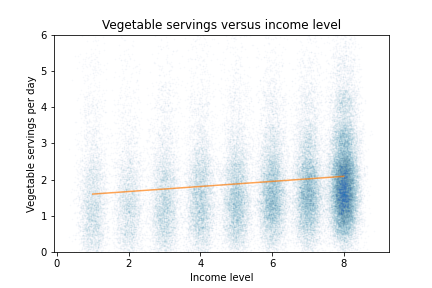
\includegraphics{chapters/figs/fig09-01.png}

The slope of the line is 0.07, which means that the difference between
the lowest and highest income brackets is about 0.49 servings per day.
So that's not a very big difference.

But it was an arbitrary choice to plot vegetables as a function of
income. We could have plotted it the other way around, like this.

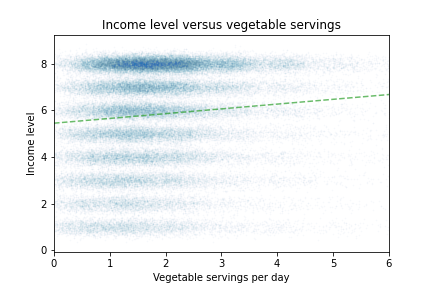
\includegraphics{chapters/figs/fig09-02.png}

The slope of this line is about 0.2, which means that the difference
between 0 and 10 servings per day is about 2 income levels, roughly from
level 5 to level 7.

And the difference between income levels 5 and 7 is about \$30,000 per
year, which is substantial.

So if we use vegetable consumption to predict income, we see a big
difference. But when we used income to predict vegetable consumption, we
saw a small difference.

This example shows that regression is not symmetric; the regression of A
onto B is not the same as the regression of B onto A.

We can see that more clearly by putting the two figures side by side and
plotting both regression lines on both figures.

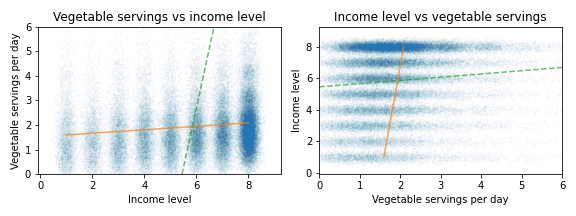
\includegraphics{chapters/figs/fig09-03.png}

They are different because they are based on different assumptions.

\begin{itemize}
\item
  On the left, we treat income as a known quantity and vegetable
  consumption as random.
\item
  On the right, we treat vegetable consumption as known and income as
  random.
\end{itemize}

When you run a regression model, you make decisions about how to treat
the data, and those decisions affect the results you get.

This example demonstrates another point, which is that regression
doesn't tell you much about causation.

\begin{itemize}
\item
  If you think people with lower income can't afford vegetables, you
  might look at the figure on the left and conclude that it doesn't make
  much difference.
\item
  If you think better diet increases income, the figure on the right
  might make you think it does.
\end{itemize}

But in general, regression can't tell you what causes what. If you see a
relationship between any two variables, A and B, the reason for the
relationship might be that A causes B, or B causes A, or there might be
other factors that cause both A and B. Regression alone can't tell you
which way it goes.

However, we have tools for quantifying relationships among multiple
variables; one of the most important is multiple regression.

\hypertarget{regression-with-statsmodels}{%
\section{Regression with
StatsModels}\label{regression-with-statsmodels}}

SciPy doesn't do multiple regression, so we'll to switch to a new
library, StatsModels. Here's the import statement.

\begin{lstlisting}[]
import statsmodels.formula.api as smf
\end{lstlisting}

For the first example, we'll load data from the Behavioral Risk Factor
Surveillance Survey (BRFSS), which we saw in the previous chapter.

\begin{lstlisting}[]
import pandas as pd

brfss = pd.read_hdf('brfss.hdf5', 'brfss')
\end{lstlisting}

Now we can use StatsModels to fit a regression model. We'll start with
one of the examples from the previous chapter, the relationship between
income and vegetable consumption. We'll check that the results from
StatsModels are the same as the results from SciPy. Then we'll move on
to multiple regression.

The function we'll use is \passthrough{\lstinline!ols!}, which stands
for ``ordinary least squares'', another name for regression.

\begin{lstlisting}[]
results = smf.ols('INCOME2 ~ _VEGESU1', data=brfss).fit()
\end{lstlisting}

The first argument is a \textbf{formula string} that specifies that we
want to regress income as a function of vegetable consumption. The
second argument is the BRFSS \passthrough{\lstinline!DataFrame!}. The
names in the formula string correspond to columns in the
\passthrough{\lstinline!DataFrame!}.

The result from \passthrough{\lstinline!ols!} is an object that
represents the model; it provides a function called
\passthrough{\lstinline!fit!} that does the actual computation.

The result is a \passthrough{\lstinline!RegressionResultsWrapper!},
which contains several attributes; the first one we'll look at is
\passthrough{\lstinline!params!}, which contains the estimated intercept
and the slope associated with \passthrough{\lstinline!\_VEGESU1!}.

\begin{lstlisting}[]
results.params
(@\dashfill@)
@@@/home/downey/miniconda3/envs/ElementsOfDataScience/lib/python3.8/site-packages/IPython/core/formatters.py:342: FutureWarning: In future versions `DataFrame.to_latex` is expected to utilise the base implementation of `Styler.to_latex` for formatting and rendering. The arguments signature may therefore change. It is recommended instead to use `DataFrame.style.to_latex` which also contains additional functionality.
  return method()@@@
\end{lstlisting}

\begin{tabular}{lr}
\midrule
{} &         0 \\
\midrule
Intercept &  5.450700 \\
\_VEGESU1  &  0.204935 \\
\midrule
\end{tabular}

The results from Statsmodels are the same as the results we got from
SciPy, so that's good!

There are only two variables in this example, so it is still simple
regression. In the next section we'll move on to multiple regression.
But first, some exercises.

\textbf{Exercise:} In the BRFSS dataset, there is a strong relationship
between vegetable consumption and income. The income of people who eat 8
servings of vegetables per day is double the income of people who eat
none, on average.

Which of the following conclusions can we draw from this data?

\begin{enumerate}
\def\labelenumi{\Alph{enumi}.}
\item
  Eating a good diet leads to better health and higher income.
\item
  People with higher income can afford a better diet.
\item
  People with high income are more likely to be vegetarians.
\end{enumerate}

\textbf{Exercise:} Let's run a regression using SciPy and StatsModels,
and confirm we get the same results.

\begin{itemize}
\item
  Compute the regression of \passthrough{\lstinline!\_VEGESU1!} as a
  function of \passthrough{\lstinline!INCOME2!} using SciPy's
  \passthrough{\lstinline!linregress()!}.
\item
  Compute the regression of \passthrough{\lstinline!\_VEGESU1!} as a
  function of \passthrough{\lstinline!INCOME2!} using StatsModels'
  \passthrough{\lstinline!smf.ols()!}.
\end{itemize}

Note: \passthrough{\lstinline!linregress!} does not handle
\passthrough{\lstinline!NaN!} values, so you will have to use
\passthrough{\lstinline!dropna!} to select the rows with valid data.

\hypertarget{multiple-regression}{%
\section{Multiple Regression}\label{multiple-regression}}

Now that we have StatsModels, getting from simple to multiple regression
is easy. As an example, we'll use data from the General Social Survey
(GSS) and we'll explore variables that are related to income.

First, let's load the GSS data.

\begin{lstlisting}[]
import pandas as pd

gss = pd.read_hdf('gss_eda.hdf', 'gss')
\end{lstlisting}

Here are the first few rows of \passthrough{\lstinline!gss!}:

\begin{lstlisting}[]
gss.head()
(@\dashfill@)
@@@/home/downey/miniconda3/envs/ElementsOfDataScience/lib/python3.8/site-packages/IPython/core/formatters.py:342: FutureWarning: In future versions `DataFrame.to_latex` is expected to utilise the base implementation of `Styler.to_latex` for formatting and rendering. The arguments signature may therefore change. It is recommended instead to use `DataFrame.style.to_latex` which also contains additional functionality.
  return method()@@@
\end{lstlisting}

\begin{tabular}{lrrrrrrrr}
\midrule
{} &  YEAR &  ID\_ &   AGE &  EDUC &  SEX &  GUNLAW &  GRASS &  REALINC \\
\midrule
0 &  1972 &    1 &  23.0 &  16.0 &    2 &     1.0 &    NaN &  18951.0 \\
1 &  1972 &    2 &  70.0 &  10.0 &    1 &     1.0 &    NaN &  24366.0 \\
2 &  1972 &    3 &  48.0 &  12.0 &    2 &     1.0 &    NaN &  24366.0 \\
3 &  1972 &    4 &  27.0 &  17.0 &    2 &     1.0 &    NaN &  30458.0 \\
4 &  1972 &    5 &  61.0 &  12.0 &    2 &     1.0 &    NaN &  50763.0 \\
\midrule
\end{tabular}

We'll start with another simple regression, estimating the parameters of
real income as a function of years of education.

\begin{lstlisting}[]
results = smf.ols('REALINC ~ EDUC', data=gss).fit()
results.params
(@\dashfill@)
@@@/home/downey/miniconda3/envs/ElementsOfDataScience/lib/python3.8/site-packages/IPython/core/formatters.py:342: FutureWarning: In future versions `DataFrame.to_latex` is expected to utilise the base implementation of `Styler.to_latex` for formatting and rendering. The arguments signature may therefore change. It is recommended instead to use `DataFrame.style.to_latex` which also contains additional functionality.
  return method()@@@
\end{lstlisting}

\begin{tabular}{lr}
\midrule
{} &             0 \\
\midrule
Intercept & -13054.459834 \\
EDUC      &   3464.463066 \\
\midrule
\end{tabular}

On the left side of the formula string,
\passthrough{\lstinline!REALINC!} is the variable we are trying to
predict; on the right, \passthrough{\lstinline!EDUC!} is the variable we
are using to inform the predictions.

The estimated slope is about \passthrough{\lstinline!3450!}, which means
that each additional year of education is associated with an additional
\$3450 of income. But income also depends on age, so it would be good to
include that in the model, too. Here's how:

\begin{lstlisting}[]
results = smf.ols('REALINC ~ EDUC + AGE', data=gss).fit()
results.params
(@\dashfill@)
@@@/home/downey/miniconda3/envs/ElementsOfDataScience/lib/python3.8/site-packages/IPython/core/formatters.py:342: FutureWarning: In future versions `DataFrame.to_latex` is expected to utilise the base implementation of `Styler.to_latex` for formatting and rendering. The arguments signature may therefore change. It is recommended instead to use `DataFrame.style.to_latex` which also contains additional functionality.
  return method()@@@
\end{lstlisting}

\begin{tabular}{lr}
\midrule
{} &             0 \\
\midrule
Intercept & -16152.855386 \\
EDUC      &   3514.291894 \\
AGE       &     54.008253 \\
\midrule
\end{tabular}

On the right side of the formula string, you can list as many variables
as you like, in this case, education and age. The
\passthrough{\lstinline!plus!} sign indicates that we expect the
contributions of the two variables to be additive, which is a common
assumption for models like this.

The estimated slope for \passthrough{\lstinline!EDUC!} is a little less
than what we saw before, about \$3514 per year.

The estimated slope for \passthrough{\lstinline!AGE!} is only about \$54
per year, which is surprisingly small.

\hypertarget{grouping-by-age}{%
\section{Grouping by Age}\label{grouping-by-age}}

To see what's going on, let's look more closely at the relationship
between income and age. We'll use a Pandas method we have not seen
before, called \passthrough{\lstinline!groupby!}, to divide the
\passthrough{\lstinline!DataFrame!} into age groups.

\begin{lstlisting}[]
grouped = gss.groupby('AGE')
type(grouped)
(@\dashfill@)
@@@pandas.core.groupby.generic.DataFrameGroupBy@@@
\end{lstlisting}

The result is a \passthrough{\lstinline!GroupBy!} object that contains
one group for each value of \passthrough{\lstinline!age!}. The
\passthrough{\lstinline!GroupBy!} object behaves like a
\passthrough{\lstinline!DataFrame!} in many ways. You can use brackets
to select a column, like \passthrough{\lstinline!REALINC!} in this
example, and then invoke a method like \passthrough{\lstinline!mean!}.

\begin{lstlisting}[]
mean_income_by_age = grouped['REALINC'].mean()
\end{lstlisting}

The result is a Pandas \passthrough{\lstinline!Series!} that contains
the mean income for each age group, which we can plot like this.

\begin{lstlisting}[]
import matplotlib.pyplot as plt

plt.plot(mean_income_by_age, 'o', alpha=0.5)
plt.xlabel('Age (years)')
plt.ylabel('Income (1986 $)')
plt.title('Average income, grouped by age');
\end{lstlisting}

\begin{center}
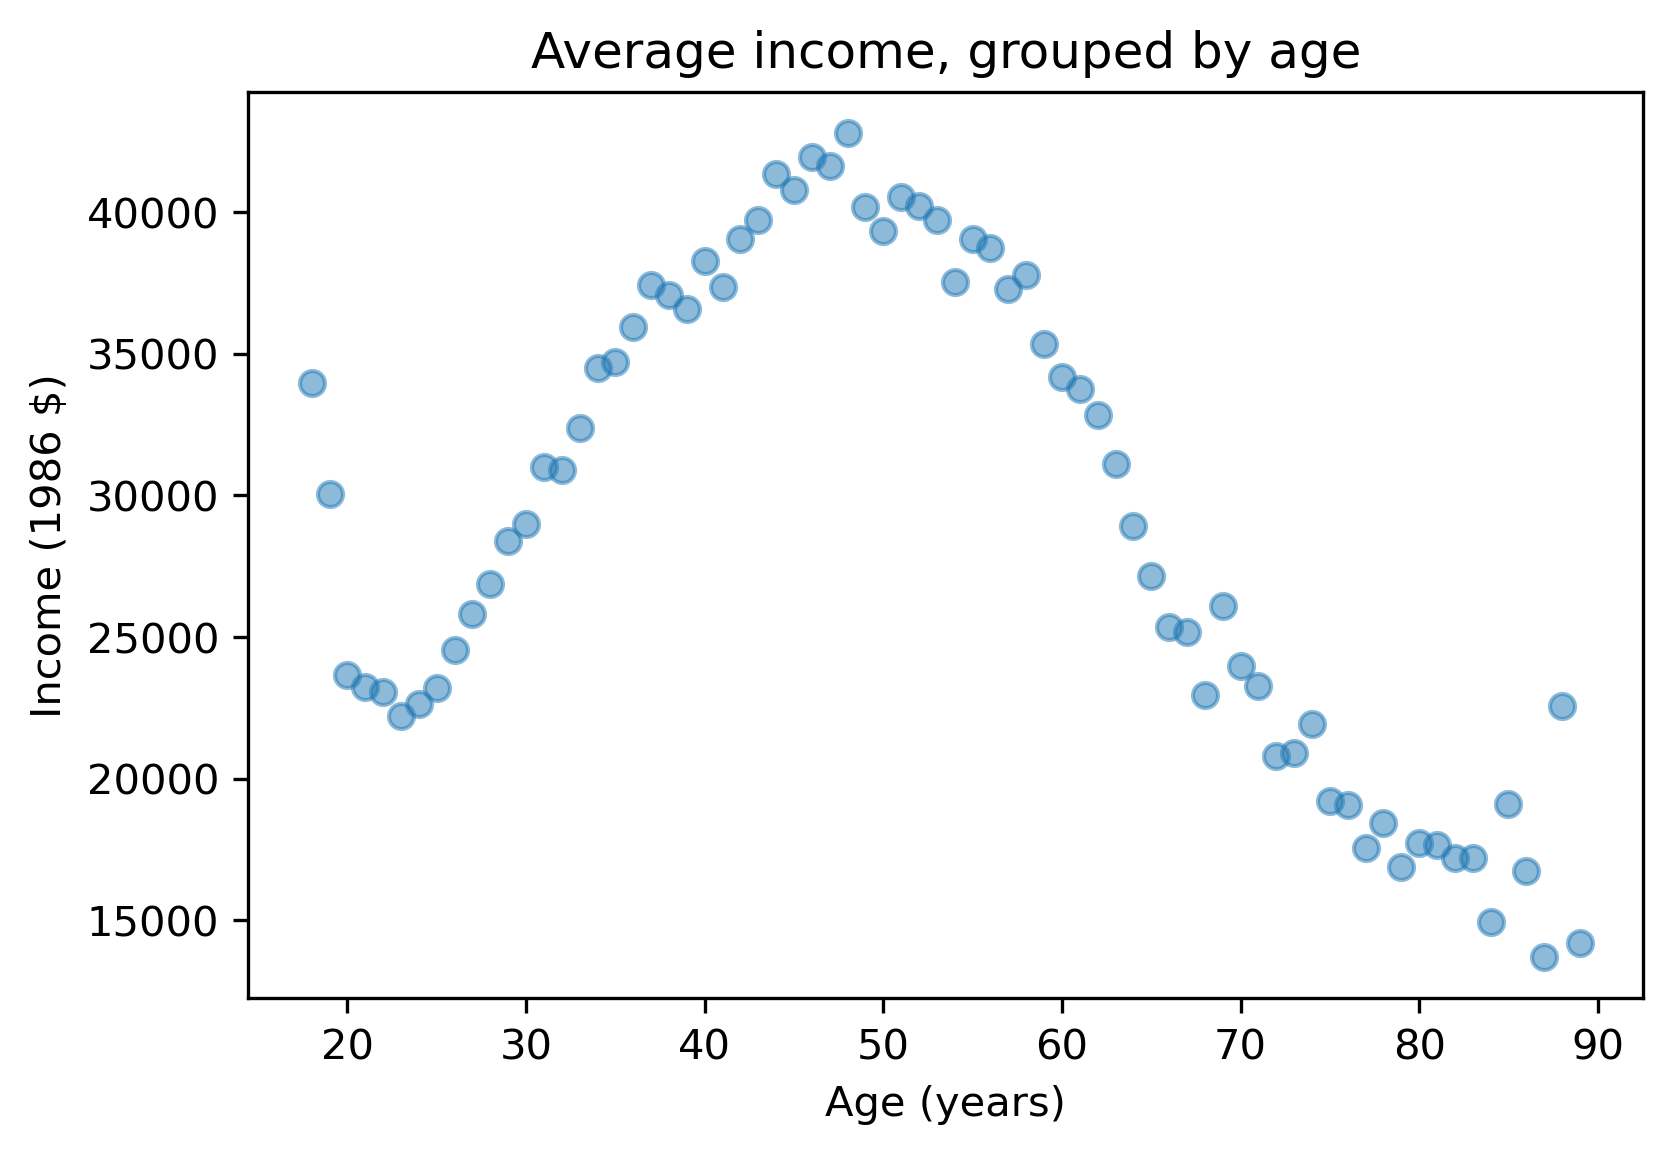
\includegraphics[width=4in]{chapters/10_regression_files/10_regression_36_0.png}
\end{center}

Average income increases from age 20 to age 50, then starts to fall.\\
And that explains why the estimated slope is so small, because the
relationship is non-linear. Remember that correlation and simple
regression can't measure non-linear relationships.

But multiple regression can! To describe a non-linear relationship, one
option is to add a new variable that is a non-linear combination of
other variables.

As an example, we'll create a new variable called
\passthrough{\lstinline!AGE2!} that equals \passthrough{\lstinline!AGE!}
squared.

\begin{lstlisting}[]
gss['AGE2'] = gss['AGE']**2
\end{lstlisting}

Now we can run a regression with both \passthrough{\lstinline!age!} and
\passthrough{\lstinline!age2!} on the right side.

\begin{lstlisting}[]
model = smf.ols('REALINC ~ EDUC + AGE + AGE2', data=gss)
results = model.fit()
results.params
(@\dashfill@)
@@@/home/downey/miniconda3/envs/ElementsOfDataScience/lib/python3.8/site-packages/IPython/core/formatters.py:342: FutureWarning: In future versions `DataFrame.to_latex` is expected to utilise the base implementation of `Styler.to_latex` for formatting and rendering. The arguments signature may therefore change. It is recommended instead to use `DataFrame.style.to_latex` which also contains additional functionality.
  return method()@@@
\end{lstlisting}

\begin{tabular}{lr}
\midrule
{} &             0 \\
\midrule
Intercept & -49865.446557 \\
EDUC      &   3293.454914 \\
AGE       &   1758.622812 \\
AGE2      &    -17.341566 \\
\midrule
\end{tabular}

In this model, the slope associated with \passthrough{\lstinline!AGE!}
is substantial, about \$1760 per year.

The slope associated with \passthrough{\lstinline!AGE2!} is about -\$17,
but that's harder to interpret.

In the next section, we'll see methods to interpret multivariate models
and visualize the results. But first, here are two exercises where you
can practice using \passthrough{\lstinline!groupby!} and
\passthrough{\lstinline!ols!}.

\textbf{Exercise:} To get a closer look at the relationship between
income and education, let's use the variable
\passthrough{\lstinline!EDUC!} to group the data, then plot mean income
in each group.

\begin{itemize}
\item
  Group \passthrough{\lstinline!gss!} by \passthrough{\lstinline!EDUC!}.
\item
  From the resulting \passthrough{\lstinline!GroupBy!} object, extract
  \passthrough{\lstinline!REALINC!} and compute the mean.
\item
  Plot mean income in each education group as a scatter plot.
\end{itemize}

What can you say about the relationship between education and income?
Does it look like a linear relationship?

\textbf{Exercise:} The graph in the previous exercise suggests that the
relationship between income and education is non-linear. So let's try
fitting a non-linear model.

\begin{itemize}
\item
  Add a column named \passthrough{\lstinline!EDUC2!} to the
  \passthrough{\lstinline!gss!} DataFrame; it should contain the values
  from \passthrough{\lstinline!EDUC!} squared.
\item
  Run a regression model that uses \passthrough{\lstinline!EDUC!},
  \passthrough{\lstinline!EDUC2!}, \passthrough{\lstinline!age!}, and
  \passthrough{\lstinline!age2!} to predict
  \passthrough{\lstinline!REALINC!}.
\end{itemize}

\hypertarget{visualizing-regression-results}{%
\section{Visualizing regression
results}\label{visualizing-regression-results}}

In the previous section we ran a multiple regression model to
characterize the relationships between income, age, and education.
Because the model includes quadratic terms, the parameters are hard to
interpret. For example, you might notice that the parameter for
\passthrough{\lstinline!EDUC!} is negative, and that might be a
surprise, because it suggests that higher education is associated with
lower income.

But the parameter for \passthrough{\lstinline!EDUC2!} is positive, and
that makes a big difference. In this section we'll see a way to
interpret the model visually and validate it against data.

Here's the model from the previous exercise.

\begin{lstlisting}[]
gss['EDUC2'] = gss['EDUC']**2

model = smf.ols('REALINC ~ EDUC + EDUC2 + AGE + AGE2', data=gss)
results = model.fit()
results.params
(@\dashfill@)
@@@/home/downey/miniconda3/envs/ElementsOfDataScience/lib/python3.8/site-packages/IPython/core/formatters.py:342: FutureWarning: In future versions `DataFrame.to_latex` is expected to utilise the base implementation of `Styler.to_latex` for formatting and rendering. The arguments signature may therefore change. It is recommended instead to use `DataFrame.style.to_latex` which also contains additional functionality.
  return method()@@@
\end{lstlisting}

\begin{tabular}{lr}
\midrule
{} &             0 \\
\midrule
Intercept & -26080.884938 \\
EDUC      &   -522.032930 \\
EDUC2     &    153.405410 \\
AGE       &   1711.838648 \\
AGE2      &    -17.128130 \\
\midrule
\end{tabular}

Sometimes we can understand a model by looking at its parameters, but
often it is better to look at its predictions.

The regression results provide a method called
\passthrough{\lstinline!predict!} that uses the model to generate
predictions. It takes a \passthrough{\lstinline!DataFrame!} as a
parameter and returns a \passthrough{\lstinline!Series!} with a
prediction for each row in the \passthrough{\lstinline!DataFrame!}. To
use it, we'll create a new \passthrough{\lstinline!DataFrame!} with
\passthrough{\lstinline!AGE!} running from 18 to 89, and
\passthrough{\lstinline!AGE2!} set to \passthrough{\lstinline!AGE!}
squared.

\begin{lstlisting}[]
import numpy as np

df = pd.DataFrame()
df['AGE'] = np.linspace(18, 89)
df['AGE2'] = df['AGE']**2
\end{lstlisting}

Next, we'll pick a level for \passthrough{\lstinline!EDUC!}, like 12
years, which is the most common value. When you assign a single value to
a column in a \passthrough{\lstinline!DataFrame!}, Pandas makes a copy
for each row.

\begin{lstlisting}[]
df['EDUC'] = 12
df['EDUC2'] = df['EDUC']**2
\end{lstlisting}

Then we can use \passthrough{\lstinline!results!} to predict the average
income for each age group, holding education constant.

\begin{lstlisting}[]
pred12 = results.predict(df)
\end{lstlisting}

The result from \passthrough{\lstinline!predict!} is a
\passthrough{\lstinline!Series!} with one prediction for each row. So we
can plot it with age on the \(x\)-axis and the predicted income for each
age group on the \(y\)-axis. And we can plot the data for comparison.

\begin{lstlisting}[]
plt.plot(mean_income_by_age, 'o', alpha=0.5)

plt.plot(df['AGE'], pred12, label='High school', color='C4')

plt.xlabel('Age (years)')
plt.ylabel('Income (1986 $)')
plt.title('Income versus age, grouped by education level')
plt.legend();
\end{lstlisting}

\begin{center}
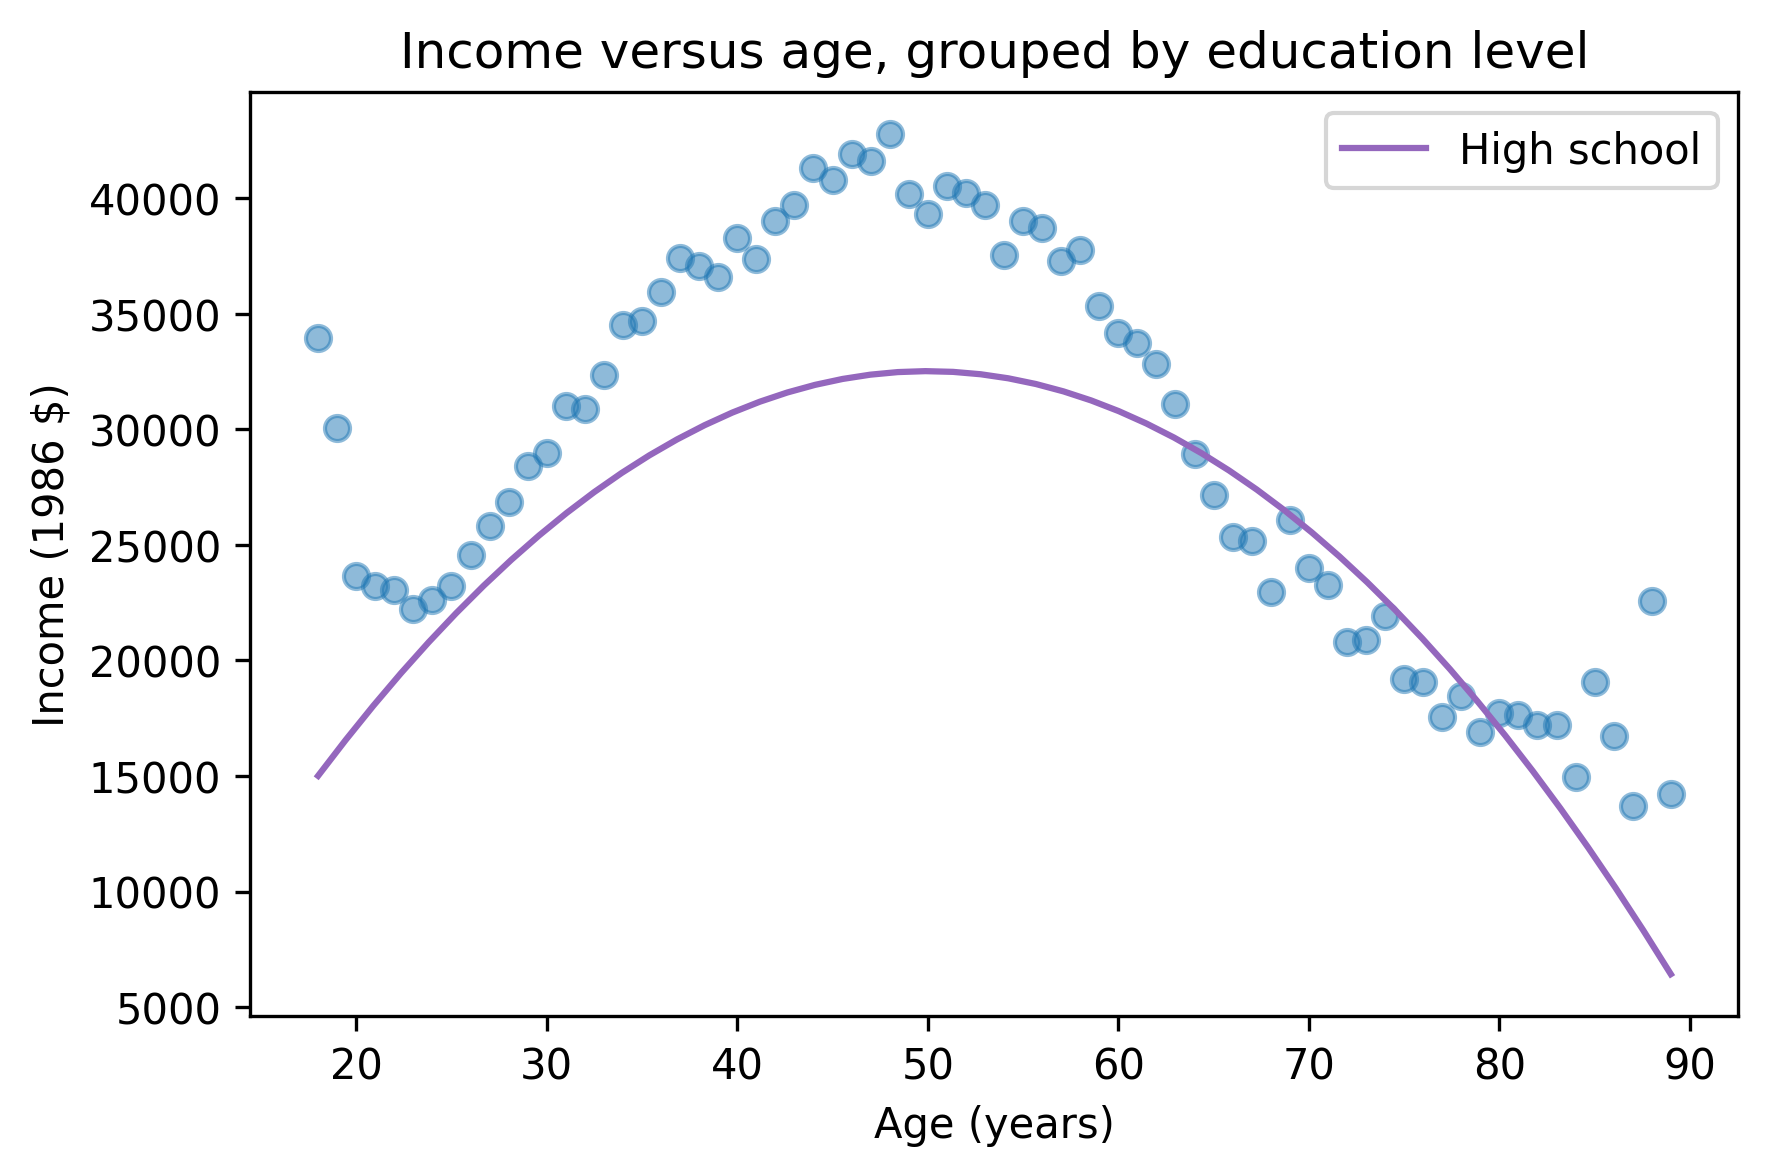
\includegraphics[width=4in]{chapters/10_regression_files/10_regression_53_0.png}
\end{center}

The dots show the average income in each age group. The line shows the
predictions generated by the model, holding education constant. This
plot shows the shape of the model, a downward-facing parabola.

We can do the same thing with other levels of education, like 14 years,
which is the nominal time to earn an Associate's degree, and 16 years,
which is the nominal time to earn a Bachelor's degree.

\begin{lstlisting}[]
df['EDUC'] = 16
df['EDUC2'] = df['EDUC']**2
pred16 = results.predict(df)

df['EDUC'] = 14
df['EDUC2'] = df['EDUC']**2
pred14 = results.predict(df)
\end{lstlisting}

\begin{lstlisting}[]
plt.plot(mean_income_by_age, 'o', alpha=0.5)

plt.plot(df['AGE'], pred16, ':', label='Bachelor')
plt.plot(df['AGE'], pred14, '--', label='Associate')
plt.plot(df['AGE'], pred12, label='High school', color='C4')

plt.xlabel('Age (years)')
plt.ylabel('Income (1986 $)')
plt.title('Income versus age, grouped by education level')
plt.legend();
\end{lstlisting}

\begin{center}
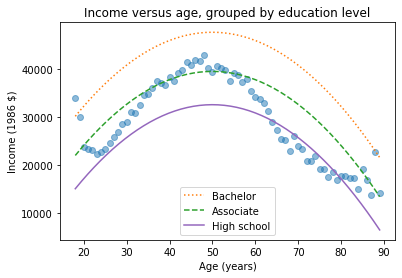
\includegraphics[width=4in]{chapters/10_regression_files/10_regression_56_0.png}
\end{center}

The lines show mean income, as predicted by the model, as a function of
age, for three levels of education. This visualization helps validate
the model, since we can compare the predictions with the data. And it
helps us interpret the model since we can see the separate contributions
of age and education.

In the exercises, you'll have a chance to run a multiple regression,
generate predictions, and visualize the results.

\textbf{Exercise:} At this point, we have a model that predicts income
using age, education, and sex.

Let's see what it predicts for different levels of education, holding
\passthrough{\lstinline!AGE!} constant.

\begin{itemize}
\item
  Create an empty \passthrough{\lstinline!DataFrame!} named
  \passthrough{\lstinline!df!}.
\item
  Using \passthrough{\lstinline!np.linspace()!}, add a variable named
  \passthrough{\lstinline!EDUC!} to \passthrough{\lstinline!df!} with a
  range of values from \passthrough{\lstinline!0!} to
  \passthrough{\lstinline!20!}.
\item
  Add a variable named \passthrough{\lstinline!AGE!} with the constant
  value \passthrough{\lstinline!30!}.
\item
  Use \passthrough{\lstinline!df!} to generate predicted income as a
  function of education.
\end{itemize}

\textbf{Exercise:} Now let's visualize the results from the previous
exercise!

\begin{itemize}
\item
  Group the GSS data by \passthrough{\lstinline!EDUC!} and compute the
  mean income in each education group.
\item
  Plot mean income for each education group as a scatter plot.
\item
  Plot the predictions from the previous exercise.
\end{itemize}

How do the predictions compare with the data?

\textbf{Optional Exercise:} Extend the previous exercise to include
predictions for a few other age levels.

\hypertarget{categorical-variables}{%
\section{Categorical Variables}\label{categorical-variables}}

Most of the variables we have used so far --- like income, age, and
education --- are numerical. But variables like sex and race are
\textbf{categorical}; that is, each respondent belongs to one of a
specified set of categories. If there are only two categories, we would
say the variable is \textbf{binary}.

With StatsModels, it is easy to include a categorical variable as part
of a regression model. Here's an example:

\begin{lstlisting}[]
formula = 'REALINC ~ EDUC + EDUC2 + AGE + AGE2 + C(SEX)'
results = smf.ols(formula, data=gss).fit()
results.params
(@\dashfill@)
@@@/home/downey/miniconda3/envs/ElementsOfDataScience/lib/python3.8/site-packages/IPython/core/formatters.py:342: FutureWarning: In future versions `DataFrame.to_latex` is expected to utilise the base implementation of `Styler.to_latex` for formatting and rendering. The arguments signature may therefore change. It is recommended instead to use `DataFrame.style.to_latex` which also contains additional functionality.
  return method()@@@
\end{lstlisting}

\begin{tabular}{lr}
\midrule
{} &             0 \\
\midrule
Intercept   & -24567.566164 \\
C(SEX)[T.2] &  -4626.727813 \\
EDUC        &   -303.398385 \\
EDUC2       &    143.954306 \\
AGE         &   1702.199322 \\
AGE2        &    -16.995151 \\
\midrule
\end{tabular}

In the formula string, the letter \passthrough{\lstinline!C!} indicates
that \passthrough{\lstinline!SEX!} is a categorical variable.

The regression treats the value \passthrough{\lstinline!SEX=1!}, which
is male, as the default, and reports the difference associated with the
value \passthrough{\lstinline!SEX=2!}, which is female. So this result
indicates that income for women is about \$4156 less than for men, after
controlling for age and education.

\hypertarget{logistic-regression}{%
\section{Logistic Regression}\label{logistic-regression}}

In the previous section, we added a categorical variables on the right
side of a regression formula; that is, we used it as a predictive
variables.

But what if the categorical variable is on the left side of the
regression formula; that is, it's the value we are trying to predict? In
that case, we can use \textbf{logistic regression}.

As an example, one of the questions in the General Social Survey asks
``Would you favor or oppose a law which would require a person to obtain
a police permit before he or she could buy a gun?'' The responses are in
a column called \passthrough{\lstinline!GUNLAW!}; here are the values.

\begin{lstlisting}[]
gss['GUNLAW'].value_counts()
(@\dashfill@)
@@@/home/downey/miniconda3/envs/ElementsOfDataScience/lib/python3.8/site-packages/IPython/core/formatters.py:342: FutureWarning: In future versions `DataFrame.to_latex` is expected to utilise the base implementation of `Styler.to_latex` for formatting and rendering. The arguments signature may therefore change. It is recommended instead to use `DataFrame.style.to_latex` which also contains additional functionality.
  return method()@@@
\end{lstlisting}

\begin{tabular}{lr}
\midrule
{} &  GUNLAW \\
\midrule
1.0 &   32038 \\
2.0 &    9975 \\
\midrule
\end{tabular}

\passthrough{\lstinline!1!} means yes and \passthrough{\lstinline!2!}
means no, so most respondents are in favor.

To explore the relationship between this variable and factors like age,
sex, and education, we can use StatsModels, which provides a function
that does logistic regression.

To use it, we have to recode the variable so \passthrough{\lstinline!1!}
means ``yes'' and \passthrough{\lstinline!0!} means ``no''. We can do
that by replacing \passthrough{\lstinline!2!} with
\passthrough{\lstinline!0!}.

\begin{lstlisting}[]
gss['GUNLAW'].replace([2], [0], inplace=True)
\end{lstlisting}

Now we can run the regression. Instead of
\passthrough{\lstinline!ols()!}, we use
\passthrough{\lstinline!logit()!}, which is named for the logit
function, which is related to logistic regression.

\begin{lstlisting}[]
formula = 'GUNLAW ~ AGE + AGE2 + EDUC + EDUC2 + C(SEX)'
results = smf.logit(formula, data=gss).fit()
(@\dashfill@)
@@@Optimization terminated successfully.
         Current function value: 0.532878
         Iterations 6@@@
\end{lstlisting}

Estimating the parameters for the logistic model is an iterative
process, so the output contains information about the number of
iterations. Other than that, everything is the same as what we have seen
before. And here are the results.

\begin{lstlisting}[]
results.params
(@\dashfill@)
@@@/home/downey/miniconda3/envs/ElementsOfDataScience/lib/python3.8/site-packages/IPython/core/formatters.py:342: FutureWarning: In future versions `DataFrame.to_latex` is expected to utilise the base implementation of `Styler.to_latex` for formatting and rendering. The arguments signature may therefore change. It is recommended instead to use `DataFrame.style.to_latex` which also contains additional functionality.
  return method()@@@
\end{lstlisting}

\begin{tabular}{lr}
\midrule
{} &         0 \\
\midrule
Intercept   &  1.347289 \\
C(SEX)[T.2] &  0.771791 \\
AGE         & -0.021314 \\
AGE2        &  0.000222 \\
EDUC        & -0.075406 \\
EDUC2       &  0.004867 \\
\midrule
\end{tabular}

The parameters are in the form of \textbf{log odds}, which you may or
may not be familiar with. I won't explain them in detail here, except to
say that positive values are associated with things that make the
outcome more likely, and negative values make the outcome less likely.

For example, the parameter associated with
\passthrough{\lstinline!SEX=2!} is 0.75, which indicates that women are
more likely to support this form of gun control. To see how much more
likely, we can generate predictions, as we did with linear regression.

As an example, we'll generate predictions for different ages and sexes,
with education held constant. First we need a
\passthrough{\lstinline!DataFrame!} with \passthrough{\lstinline!AGE!}
and \passthrough{\lstinline!EDUC!}.

\begin{lstlisting}[]
df = pd.DataFrame()
df['AGE'] = np.linspace(18, 89)
df['EDUC'] = 12
\end{lstlisting}

Then we can compute \passthrough{\lstinline!AGE2!} and
\passthrough{\lstinline!EDUC2!}.

\begin{lstlisting}[]
df['AGE2'] = df['AGE']**2
df['EDUC2'] = df['EDUC']**2
\end{lstlisting}

We can generate predictions for men like this.

\begin{lstlisting}[]
df['SEX'] = 1
pred1 = results.predict(df)
\end{lstlisting}

And for women like this.

\begin{lstlisting}[]
df['SEX'] = 2
pred2 = results.predict(df)
\end{lstlisting}

Now, to visualize the results, we'll start by plotting the data. As
we've done before, we'll divide the respondents into age groups and
compute the mean in each group. The mean of a binary variable is the
fraction of people in favor.

Then we can plot the predictions, for men and women, as a function of
age.

\begin{lstlisting}[]
grouped = gss.groupby('AGE')
favor_by_age = grouped['GUNLAW'].mean()
plt.plot(favor_by_age, 'o', alpha=0.5)

plt.plot(df['AGE'], pred2, label='Female')
plt.plot(df['AGE'], pred1, '--', label='Male')

plt.xlabel('Age')
plt.ylabel('Probability of favoring gun law')
plt.title('Support for gun law versus age, grouped by sex')
plt.legend();
\end{lstlisting}

\begin{center}
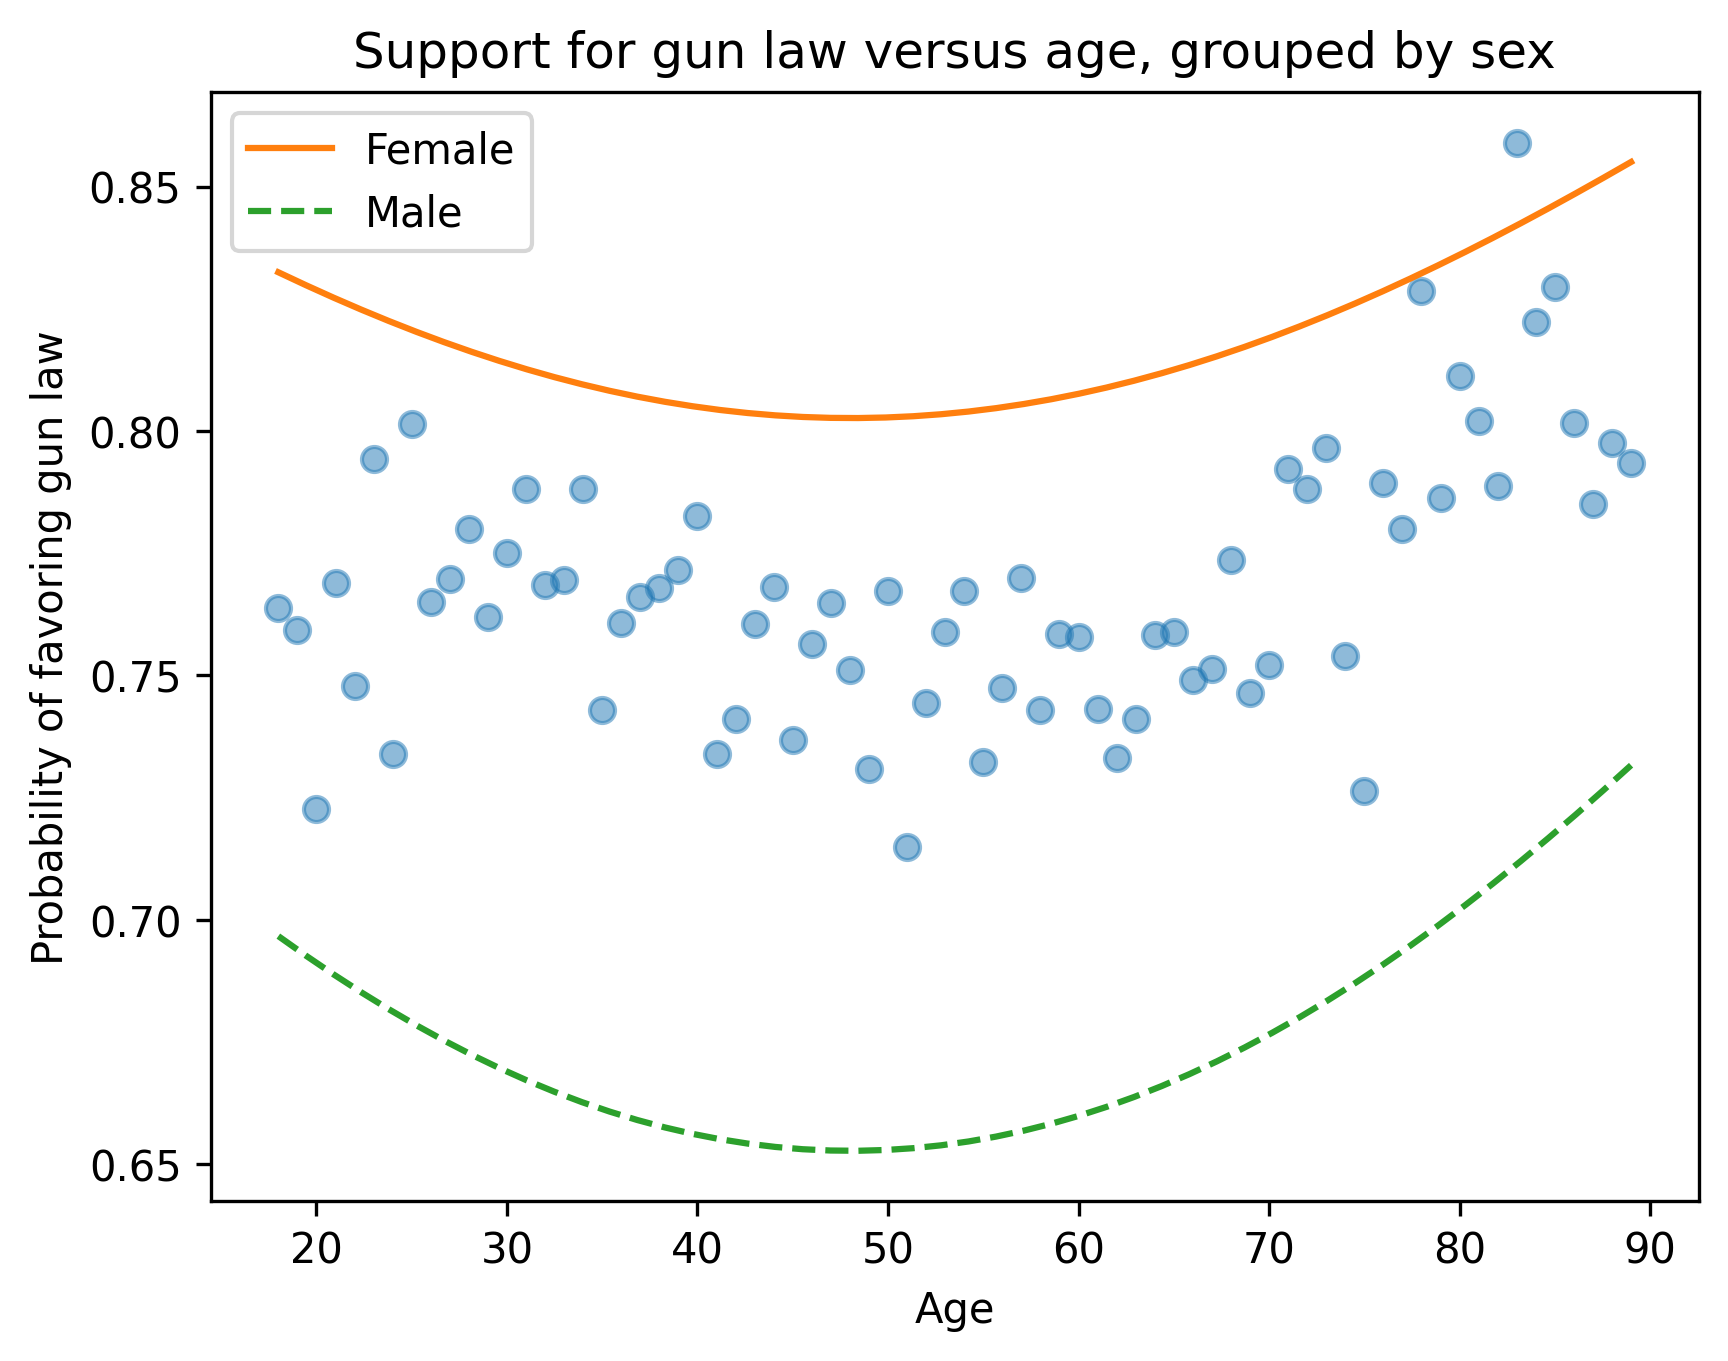
\includegraphics[width=4in]{chapters/10_regression_files/10_regression_83_0.png}
\end{center}

According to the model, people near age 50 are least likely to support
gun control (at least as this question was posed). And women are more
likely to support it than men, by almost 15 percentage points.

Logistic regression is a powerful tool for exploring relationships
between a binary variable and the factors that predict it. In the
exercises, you'll explore the factors that predict support for
legalizing marijuana.

\textbf{Exercise:} Let's use logistic regression to predict a binary
variable. Specifically, we'll use age, sex, and education level to
predict support for legalizing marijuana in the U.S.

In the GSS dataset, the variable \passthrough{\lstinline!GRASS!} records
the answer to the question ``Do you think the use of marijuana should be
made legal or not?''

\begin{enumerate}
\def\labelenumi{\arabic{enumi}.}
\item
  First, use \passthrough{\lstinline!replace!} to recode the
  \passthrough{\lstinline!GRASS!} column so that
  \passthrough{\lstinline!1!} means yes and \passthrough{\lstinline!0!}
  means no. Use \passthrough{\lstinline!value\_counts!} to check.
\item
  Next, use \passthrough{\lstinline!smf.logit()!} to predict
  \passthrough{\lstinline!GRASS!} using the variables
  \passthrough{\lstinline!AGE!}, \passthrough{\lstinline!AGE2!},
  \passthrough{\lstinline!EDUC!}, and \passthrough{\lstinline!EDUC2!},
  along with \passthrough{\lstinline!SEX!} as a categorical variable.
  Display the parameters. Are men or women more likely to support
  legalization?
\item
  To generate predictions, start with an empty DataFrame. Add a column
  called \passthrough{\lstinline!AGE!} that contains a sequence of
  values from 18 to 89. Add a column called
  \passthrough{\lstinline!EDUC!} and set it to 12 years. Then compute a
  column, \passthrough{\lstinline!AGE2!}, which is the square of
  \passthrough{\lstinline!AGE!}, and a column,
  \passthrough{\lstinline!EDUC2!}, which is the square of
  \passthrough{\lstinline!EDUC!}.
\item
  Use \passthrough{\lstinline!predict!} to generate predictions for men
  (\passthrough{\lstinline!SEX=1!}) and women
  (\passthrough{\lstinline!SEX=2!}).
\item
  Generate a plot that shows (1) the average level of support for
  legalizing marijuana in each age group, (2) the level of support the
  model predicts for men as a function of age, and (3) the level of
  support predicted for women as a function of age.
\end{enumerate}

\hypertarget{summary}{%
\section{Summary}\label{summary}}

At this point, I'd like to summarize the topics we've covered so far,
and make some connections that might clarify the big picture.

A central theme of this book is \textbf{exploratory data analysis},
which is a process and set of tools for exploring a dataset, visualizing
distributions, and discovering relationships between variables. The last
four chapters demonstrate the steps of this process:

\begin{itemize}
\item
  Chapter 7 is about importing and cleaning data, and checking for
  errors and other special conditions. This might not be the most
  exciting part of the process, but time spent validating data can save
  you from embarrassing errors.
\item
  Chapter 8 is about exploring variables one at a time, visualizing
  distributions using PMFs, CDFs, and KDE, and choosing appropriate
  summary statistics.
\item
  In Chapter 9 we explored relationships between variables two at a
  time, using scatter plots and other visualizations; and we quantified
  those relationships using correlation and simple regression.
\item
  Finally, in this chapter, we explored multivariate relationships using
  multiple regression and logistic regression.
\end{itemize}

In Chapter 7, we looked at the distribution of birth weights from the
National Survey of Family Growth. If you only remember one thing,
remember the 99 pound babies, and how much it can affect your results if
you don't validate the data.

In Chapter 8 we looked at the distributions of age, income, and other
variables from the General Social Survey. I recommended using CDFs as
the best way to explore distributions. But when you present to audiences
that are not familiar with CDFs, you can use PMFs if there are a small
number of unique values, and KDE if there are a lot.

In Chapter 9 we looked at heights and weights from the BRFSS, and
developed several ways to visualize relationships between variables,
including scatter plots, violin plots, and box plots.

We used the coefficient of correlation to quantify the strength of a
relationship. We also used simple regression to estimate slope, which is
often what we care more about, not correlation.

But remember that both of these methods only capture linear
relationships; if the relationship is non-linear, they can be
misleading. Always look at a visualization, like a scatter plot, before
computing correlation or simple regression.

In Chapter 10 we used multiple regression to add control variables and
to describe non-linear relationships. And finally we used logistic
regression to explain and predict binary variables.

We moved through a lot of material quickly, but if you practice and
apply these methods to other questions and other datasets, you will
learn more as you go.

In the next chapter, we will move on to a new topic, resampling, which
is a versatile tool for statistical inference.

